\documentclass{article}
\usepackage[utf8]{inputenc}
\usepackage{amsmath}
\usepackage{amsfonts}
\usepackage{tikz}
\usepackage{tkz-euclide}
\usepackage{graphicx}
\graphicspath{ {./images/} }

\begin{document}

\begin{center}
        \section*{Maths Problems Set 4 (16 February 2020)}
\end{center}

\begin{enumerate}
    \item
    5 points are placed in a $1\times1$ square. Show that no matter where the points are placed there will always be a pair of points with a distance of less than or equal to $\frac{1}{\sqrt{2}}$ between them.

    
    \item
    A positive integer ends in the digit 4 and has the property that it becomes four times as large when the 4 is moved from the end and placed at the front. What is the smallest such number?
    
    \item
    I have two identical but non-uniform ropes. I know that if I light one end of either rope it will burn for exactly one hour. How can I time 45 minutes? (I have a lighter of some sort).
    
    \item
    The minute and hour hands on a analog clock overlap at 12 o’clock. Where else do they overlap?
    
    \item
    Two quarter circles are inscribed in a square of side length 1 as shown in the diagram below. A circle is then inscribed as shown. Find the radius of the circle.
    
    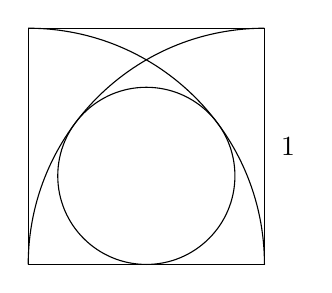
\begin{tikzpicture}[scale=3]
        \draw (0, 0) -- (0, 1) -- (1, 1) -- (1, 0) -- cycle;
        \draw (1, 0) arc[start angle=0, end angle=90, radius=1];
        \draw (1, 1) arc[start angle=90, end angle=180, radius=1];
        \node[label] at (1.1, 0.5) {1};
        \draw (0.5, 3/8) circle [radius=3/8];
    \end{tikzpicture}
    
    \item
    You visit a remote desert island inhabited by one hundred very friendly dragons,all of whom have green eyes. They haven’t seen a human for many centuries andare very excited about your visit. They show you around their island and tell youall about their dragon way of life (dragons can talk, of course).They seem to be quite normal, as far as dragons go, but then you find outsomething rather odd. They have a rule on the island which states that if a dragonever finds out that he/she has green eyes, then at precisely midnight on the day ofthis discovery, he/she must relinquish all dragon powers and transform into a long-tailed sparrow. However, there are no mirrors on the island, and they never talkabout eye color, so the dragons have been living in blissful ignorance throughoutthe ages.Upon your departure, all the dragons get together to see you off, and in a tearfulfarewell you thank them for being such hospitable dragons. Then you decide to tellthem something that they all already know (for each can see the colors of the eyes ofthe other dragons). You tell them all that at least one of them has green eyes. Thenyou leave, not thinking of the consequences (if any). Assuming that the dragons are(of course) infallibly logical, what happens?If something interesting does happen, what exactly is the new information thatyou gave the dragons? % https://projects.iq.harvard.edu/files/phys_prob2.pdf

    \item
    For what $x$ is $\sin(x) + \cos(x) \geq 1$
    
    
    \item
    Evaluate $\int \limits_{-\pi}^{\pi} |\sin x + \cos x|\text{ }\mathrm{d}x$.
    
    \item
    Find $\int \sec x \text{ }\mathrm{d}x$ and $\int \mathrm{cosec} x \text{ }\mathrm{d}x$.
    
    \item
    You are walking along a route in a city with square blocks. You need to travel six blocks North and and six blocks East. The shortest possible route is therefore twelve blocks. How many different such twelve-block routes exist?
    
    \item
    Evaluate $\int \limits_{0}^{1} (1-\sqrt{x})^n \text{ }\mathrm{d}x$.
    
    \item
    
    \item
    In Secret Santa, a group of people each pick out the name of a single other person at random, such that no one picks out their own name. In a Secret Santa group of $n$ people, find in terms of $n$ the probability that everyone picks out the same person that picked them.
            
    \item
    Timmy the gnome lives at the end of Exponential Road. Exponential Road is a road up a mountain that matches a segment of the graph $y = e^x$. Exponential Road starts at a gradient of 0.0025 and ends with gradient 8. One day Timmy the gnome was wandering home, starting at the beginning of Exponential Road. How long is the path Timmy takes to travel home?

    
    \item
    Newton's law of cooling states that the rate of heat transfer of a body is directly proportional to the difference between the temperature of the body and that of its surroundings. This leads the objects to tend towards the same temperature. A can of Coke with temperature 15 degrees is placed in a fridge kept at constant temperature of 5 degrees. Given that it takes 2 minutes for the can of coke to reach 10 degrees how long does it take to reach a temperature of 7.5 degrees?
    
    \item
    
    \item


    
    
    
    
    
    
\end{enumerate}



\end{document}
